
% Suppose $p < \infty$ and we wish to choose a $\phi$ to change $\pbase$ into
% $\palt$, for which \defref{prior_nl_pert} gives that we must choose
% %
% \begin{align}\eqlabel{phi_for_palt}
% %
% \phi(\theta) = \alpha \palt(\theta)^{1/p} - \pbase(\theta)^{1/p}
%     \mathtxt{where}\alpha > 0.
% %
% \end{align}
%
As long as $\palt(\nu) > 0$ whenever $\pbase(\nu) >
0$ (a condition which is certainly not always satisfied), one can choose
%
\begin{align*}
%
\alpha = \sup_{\nu} \left(\frac{\pbase(\nu)}{\palt(\nu)}\right)^{1/p}
%
\end{align*}
%
to guarantee that $\phi(\nu)$ is non-negative.  However, by doing so, one might
have to create a ``large'' perturbation, according to the $\norm{\cdot}_p$,
as the following \exref{positive_pert_large} demonstrates.

% %%%%%%%%%%%%%%%%%%%%%%%%%%%%%%%%%%%%%%%%%%%%%%%%%%%%%%%%%%%%%%%%%%%%%%%%%
% \begin{ex}
% %
% Let $\pbase(\nu) = \frac{4}{3}\ind{\frac{1}{4} \le \nu \le 1}$ and $\palt(\nu) =
% \frac{4}{3}\ind{0 \le \nu \le \frac{3}{4}}$.  Then, for any $\alpha > 0$, any $1
% \le p < \infty$, and for $\phi$ as given in \eqref{phi_for_palt}, $\phi(7/8) <
% 0$.  So there is no value of $\alpha$ that can transform $\pbase$ into $\palt$
% using only a positive perturbation.
% %
% \end{ex}
%%%%%%%%%%%%%%%%%%%%%%%%%%%%%%%%%%%%%%%%%%%%%%%%%%%%%%%%%%%%%%%%%%%%%%%%%
%%%%%%%%%%%%%%%%%%%%%%%%%%%%%%%%%%%%%%%%%%%%%%%%%%%%%%%%%%%%%%%%%%%%%%%%%

\SimPositivePertFig

%%%%%%%%%%%%%%%%%%%%%%%%%%%%%%%%%%%%%%%%%%%%%%%%%%%%%%%%%%%%%%%%%%%%%%%%%
\begin{ex}\exlabel{positive_pert_large}
%

%%%%%%%%%%%%%%%%%%%%%%%%%%%%%%%%%%%%%%%%%%%%%%%%%%%%%%%%%%%%%%%%%%%%%%%%%
%%%%%%%%%%%%%%%%%%%%%%%%%%%%%%%%%%%%%%%%%%%%%%%%%%%%%%%%%%%%%%%%%%%%%%%%%
% \begin{figure}[h!]
%
% 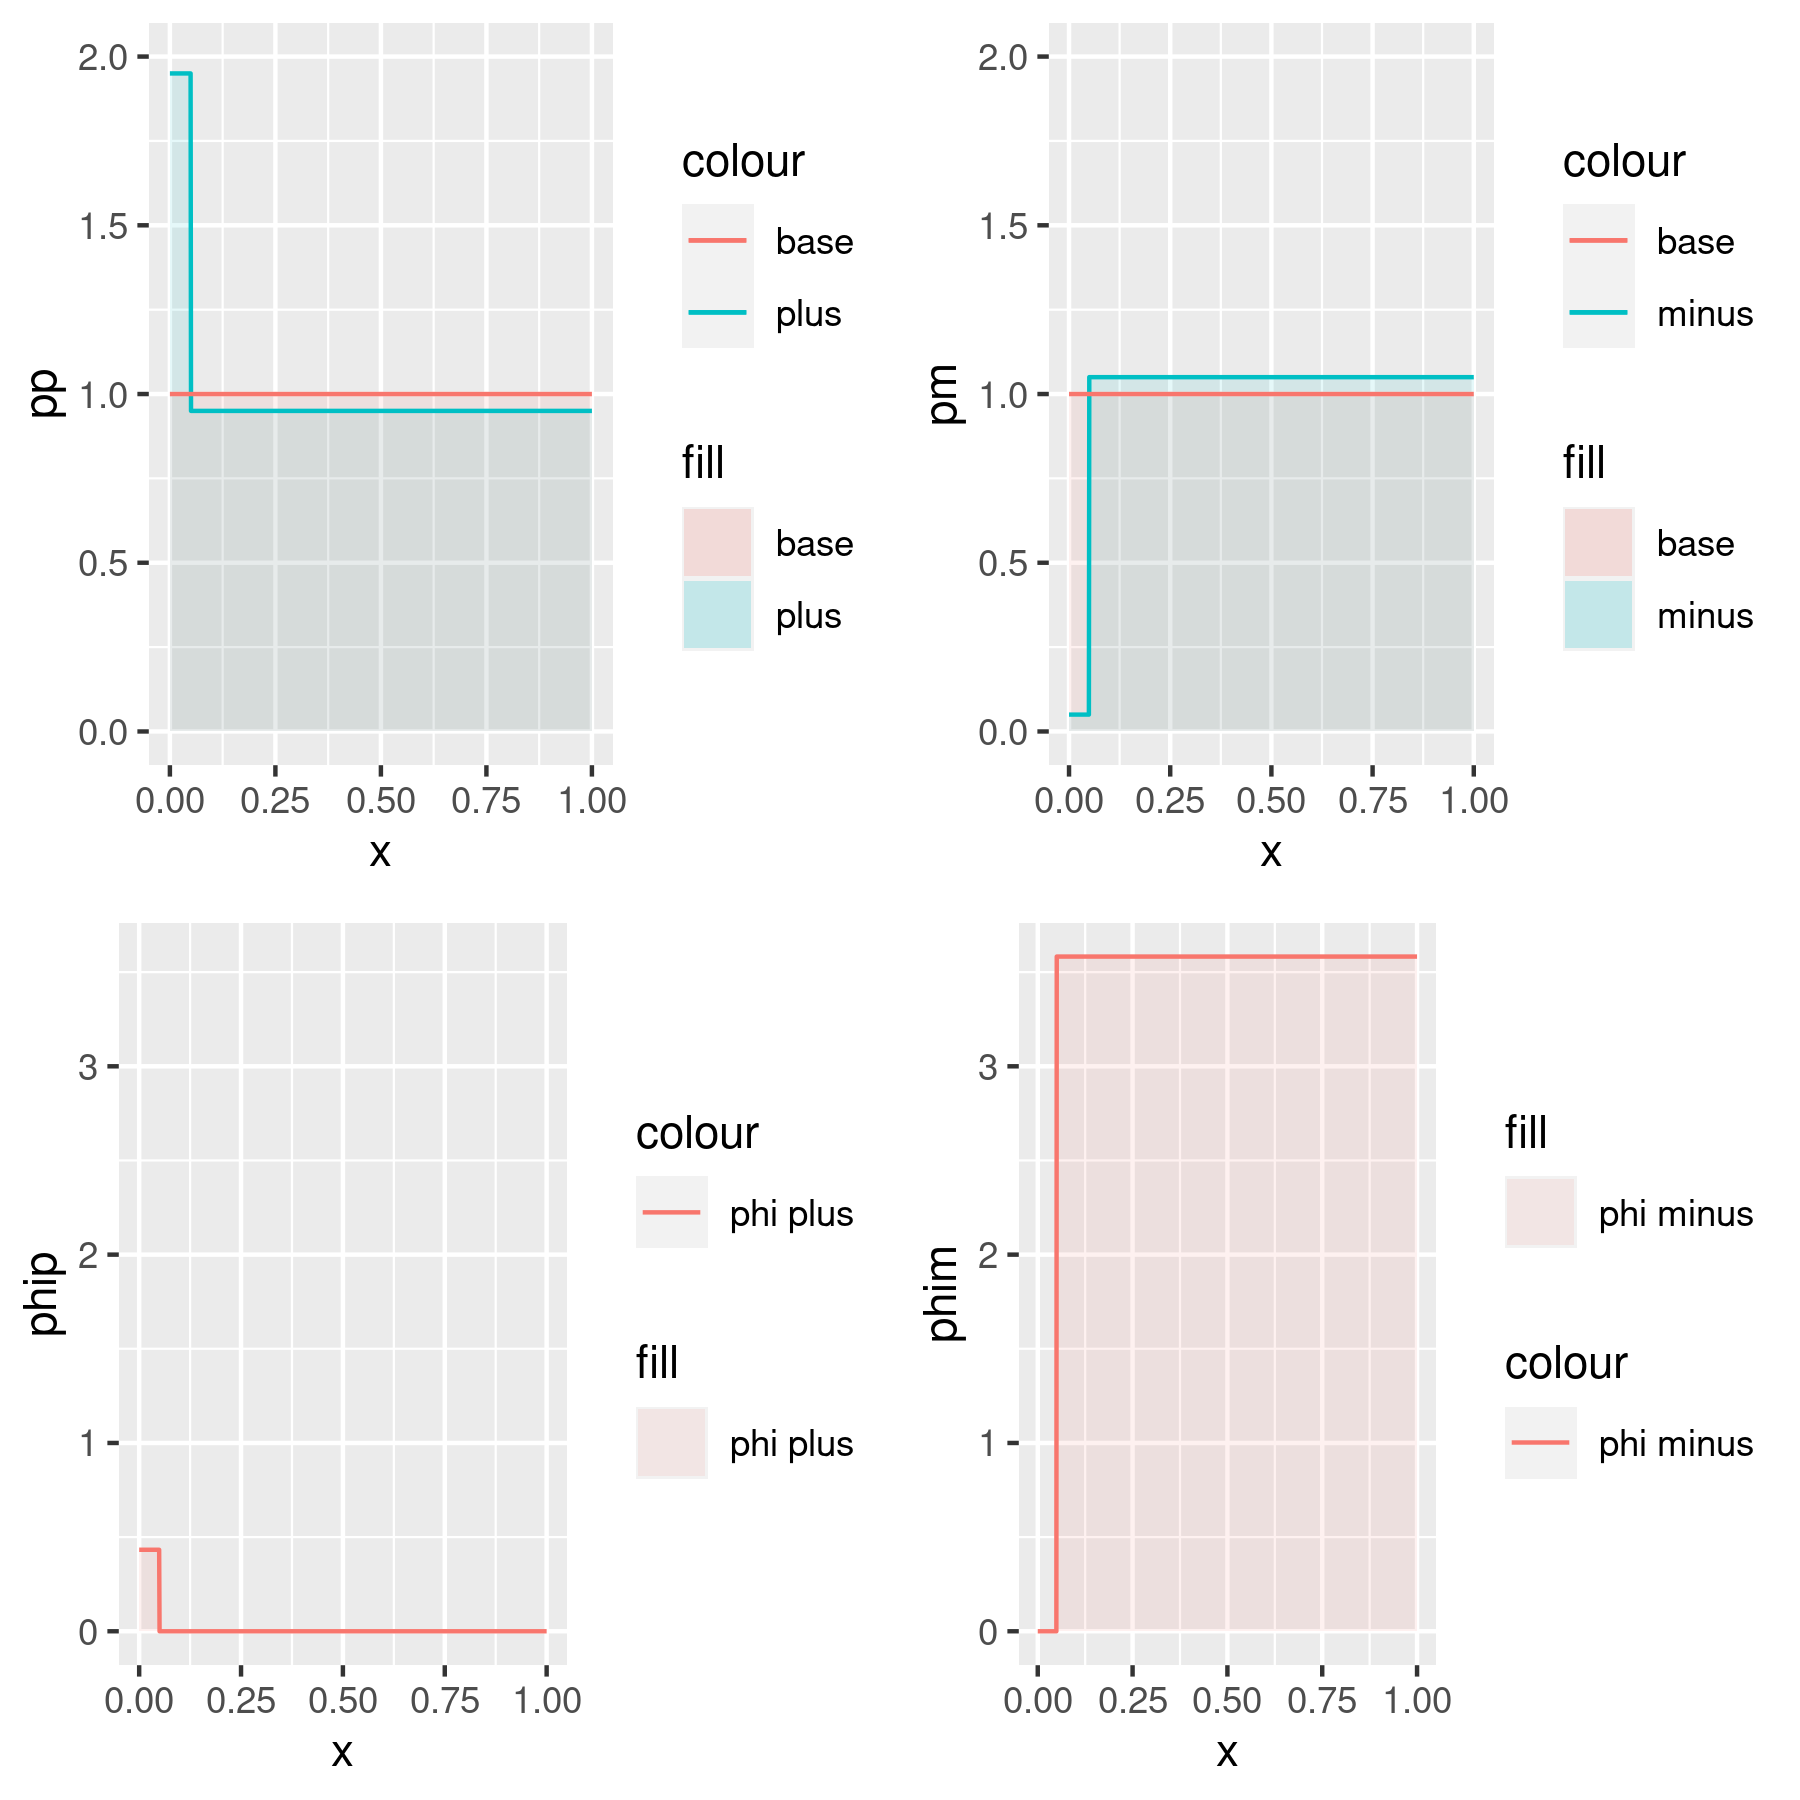
\includegraphics[width=0.980\linewidth,height=0.980\linewidth]{static_images/positive_phi_example.png}
% %
% \caption{A plot of the perturbations from \exref{positive_pert_large}
% with $p=2$ and $\epsilon=0.05$.  Positive $\phi$ can only add mass, so to remove
% a small amount of mass requires adding mass everywhere else and re-normalizing,
% resulting in a large perturbation according to $\norm{\cdot}_p$.}
% %
% \figlabel{positive_pert_large}
% \centering
% \end{figure}
%%%%%%%%%%%%%%%%%%%%%%%%%%%%%%%%%%%%%%%%%%%%%%%%%%%%%%%%%%%%%%%%%%%%%%%%%

Let $\pbase(\nu) = \ind{0 \le \nu \le 1}$.  For some $\delta > 0$ and $0 <
\epsilon \ll 1$, let
%
\begin{align*}
%
\palt(\nu) :={}&
    \left(\frac{1-\delta \epsilon}{1 - \epsilon} \right)
        \ind{\epsilon \le \nu \le 1} +
    \delta \ind{0 \le \nu \le \epsilon}.
%
\end{align*}
%
% where the final approximation is due to the smallness of $\epsilon$.
Then (PHI FOR PALT) gives, for some $\alpha$,
%
\begin{align*}
%
\phi ={}&
    \left( \alpha\left(\frac{1-\delta \epsilon}{1-\epsilon} \right)^{1/p}
        - 1
    \right)
        \ind{\epsilon \le \nu \le 1} +
    \left(\alpha \delta^{1/p} - 1 \right) \ind{0 \le \nu \le \epsilon}.
%
%
\end{align*}
%
And
%
\begin{align*}
%
\norm{\phi}_p ={}&
    \left( \alpha\left(\frac{1-\delta \epsilon}{1-\epsilon} \right)^{1/p} - 1
    \right) (1- \epsilon) +
    \left(\alpha \delta^{1/p} - 1 \right) \epsilon.
%
\end{align*}
%
For $\phi$ to be positive, we require
%
\begin{align*}
%
\alpha^p \ge \frac{1 - \epsilon}{1 - \delta \epsilon}
    \mathtxt{and}
\alpha^p \ge \frac{1}{\delta}.
%
\end{align*}

First, let us consider adding a small amount of prior mass, taking $\delta = 2 -
\epsilon$; let the corresponding perturbation be $\phi^+$.  For $\delta > 1$,
then we achieve $\phi \ge 0$ by taking $\alpha^p = \frac{1 - \epsilon}{1 -
\delta \epsilon}$.  Using the fact that $\epsilon \ll 1$ and keeping only
leading-order terms,
%
\begin{align*}
%
\frac{1-\epsilon}{1 - \delta \epsilon} \approx{}&
    (1- \epsilon)(1 + \delta \epsilon)
\\\approx{}& 1 + (\delta - 1) \epsilon
\\\approx{}& 1 + \epsilon,
%
\end{align*}
%
so
%
\begin{align*}
%
\norm{\phi^+}_p  ={}&
    \left(\alpha \delta^{1/p} - 1 \right) \epsilon
\\\approx{}&
    \left(
        \left( \left(1 + \epsilon\right) \left(2 - \epsilon \right)\right)^{1/p}
        - 1 \right) \epsilon
\\\approx{}&
%
\left( 2^{1/p} - 1 \right) \epsilon.
%
\end{align*}
%

Next, consider removing the same amount of mass with the symmetric change
$\delta = \epsilon$, letting $\phi^-$ be the corresponding perturbation. Then we
can ensure that $\phi(\nu) \ge 0$ with $\alpha^p \ge \epsilon^{-1}$, and
$\epsilon \ll 1$ gives
%
\begin{align*}
%
\frac{1-\delta\epsilon}{1 - \epsilon} \approx{}& 1- \epsilon,
%
\end{align*}
%
and
%
\begin{align*}
%
\norm{\phi^-}_p  ={}&
    \left( \alpha\left(\frac{1-\delta \epsilon}{1-\epsilon} \right)^{1/p} - 1
    \right) (1- \epsilon)
\\\approx{}&
\left(\left(\frac{1- \epsilon}{\epsilon}  \right)^{1/p} - 1\right)(1 - \epsilon)
%
\\\approx{}&
    \left( \frac{1}{\epsilon}\right)^{1/p}.
%
\end{align*}

Since $\epsilon$ is small, $\norm{\phi^-}_p \approx \left(
\frac{1}{\epsilon}\right)^{1/p} \gg \norm{\phi^+}_p \approx \left( 2^{1/p} - 1
\right) \epsilon$, despite the two perturbations respectively removing and
adding the same amount of arbitrarily small probability mass.

\end{ex}
%%%%%%%%%%%%%%%%%%%%%%%%%%%%%%%%%%%%%%%%%%%%%%%%%%%%%%%%%%%%%%%%%%%%%%%%%
